\documentclass{article}                     % onecolumn (standard format)

\usepackage{graphicx}
\usepackage{float}
\usepackage{amsmath}
\usepackage{cite}
\usepackage{subcaption}
\usepackage{rotating}
\usepackage[left=2.2cm, right=2.2cm]{geometry}
\usepackage{algpseudocode}
\usepackage{algorithm}
%\floatstyle{ruled}
\usepackage[hidelinks]{hyperref}
\usepackage{algpseudocode}


\newfloat{algorithm}{tbp}{loa}
\providecommand{\algorithmname}{Algorithm}
\floatname{algorithm}{\protect\algorithmname}


%\renewcommand{\thesection}{\Roman{section}}
\usepackage{titlesec}
\titleformat{\section}
{\normalfont\Large\bfseries}{Exercise~\thesection}{1em}{}

\newfloat{algorithm}{tbp}{loa}
\providecommand{\algorithmname}{Algorithm}
\floatname{algorithm}{\protect\algorithmname}

\newcommand{\nt}[1]{\neg #1}
%
% \usepackage{mathptmx}      % use Times fonts if available on your TeX system
%
% insert here the call for the packages your document requires
%\usepackage{latexsym}
% etc.
%
% please place your own definitions here and don't use \def but
% \newcommand{}{}
%

%
\begin{document}
	
	\title{Introduction to AI - assignment 3}
	
	
	\author{Oded~Yechiel}
	
	\date{27/11/18}
	
	\maketitle
	\tableofcontents
	\section{Agents and environment simulators}
	\subsection{An agent that plays Whist}
	Whist is a zero-sum adversarial game. The environment is static and discrete, non observed and non deterministic. There are many possible goal states, and the agent should maximize its own performance while minimizing the performance of the adversarial agent. Therefore, a \textbf{utility-based agent} will best assess the situation and provide the ultimate action.
	\subsection{An agent that can solve Sokoban problems}
	Sokoban is a single player puzzle-like game with a single goal state. The environment is static, discrete, fully observable and deterministic. Therefore, a \textbf{goal-based agent} will be most suitable than all other agents.
	\subsection{An autonomous humanoid robot that can win the DARPA robotics challenge}
	The DRC's task require the robot to perform a series of tasks. Although points are distributed per task, such as, go through the gate, enter the car, drive the car and exit the car, these are merely subgoals and are sequential. Therefore, it would be most logical of using a \textbf{goal-based agent}. The environment is static, continuous, discrete and partially observable.
	\subsection{An internet shopping agent specializing in trip planning}
	An internet shopping agent has many goals, with various optimizing criteria, such as time, cost and comfort. The environment \textbf{may be} considered as a deterministic, fully observable (after query the agent has all of the information) single operating agent (assuming tickets are not running out). Since there is no one perfect goal, the agent should be \textbf{utility-based agent.}
	\subsection{An agent that can play Go}
	Go is a fully observable, non-deterministic, static adversarial game. Although there is only one winner and a definite goal state, it is unlikely for any agent to calculate so deeply into the game and find the optimal action. Therefore, for a given action it is required to assess the situation and decide what action is sub-optimal for the problem. Therefore, a \textbf{utility-based agent} is advised.
	
	\section{Search}
	In the hurricane environment, shown in Fig.~\ref{fig:environment}, there are many different ways in which it is possible to calculate the heuristics of an action. The half-star heuristic, $ h' $ calculates the performance by locating the vertex with most un-savable people and multiplying them by a large number. In this exercise  we shall multiply each person by 100 for ease of calculation and distinction, although multiplying by the "Deadline value" is sufficient.
	
	\begin{figure}
		\centering
		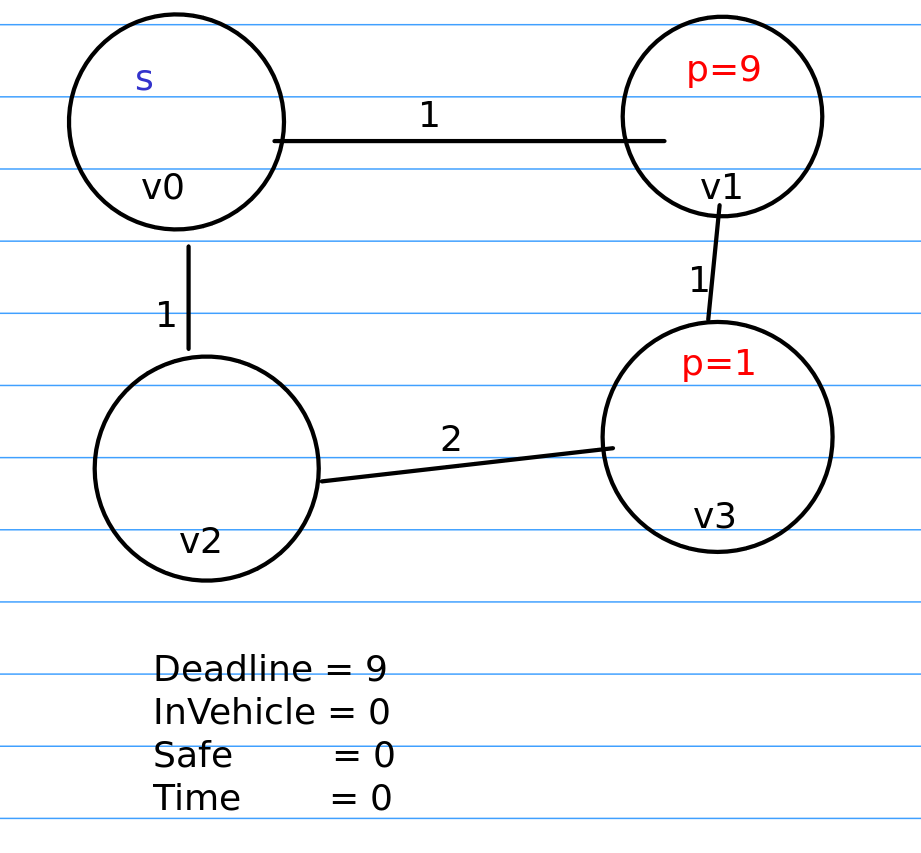
\includegraphics[width=0.5\linewidth]{environment}
		\caption{The hurricane environment.}
		\label{fig:environment}
	\end{figure}
	
	
	We can examine an example of calculating the heuristics for the starting location. The agent is at $ V_0 $ and it is possible to go to $ V_1 $ or $ V_2 $. The heuristic for going to $ V_1 $ will be 100, since we have picked up all the 9 people in $ V_1 $ and the only town with people is $ V_3 $ with 1 person. Going to $ V_2 $ will result in a heuristic of 900, since in $ V_1 $ there are 9 people which are un-savable.
	
	\textbf{NOTE - } this heuristic is not admissible! In the assignment we have used a different heuristic which is admissible where all of the people are taken into account, not only the people in the town with most people.
	
	
	\subsection{Greedy agent}
	From the example above, the greedy agent will obviously prefer going to $ V_1 $, even-though it is obvious that the pick-up will be his final move. Fig. \ref{fig:q2a} shows the decision making of the greedy agent: $ V_0 \rightarrow V_1 \rightarrow V_3 $.
	
	The greedy agent relies on an extremely optimistic heuristic that assumes that whoever in the vehicle will get to safety, and does not take those people (the ones in the vehicle) into account in the calculation. Therefore, the result of the greedy agent is not optimal.
	
	\begin{figure}
		\centering
		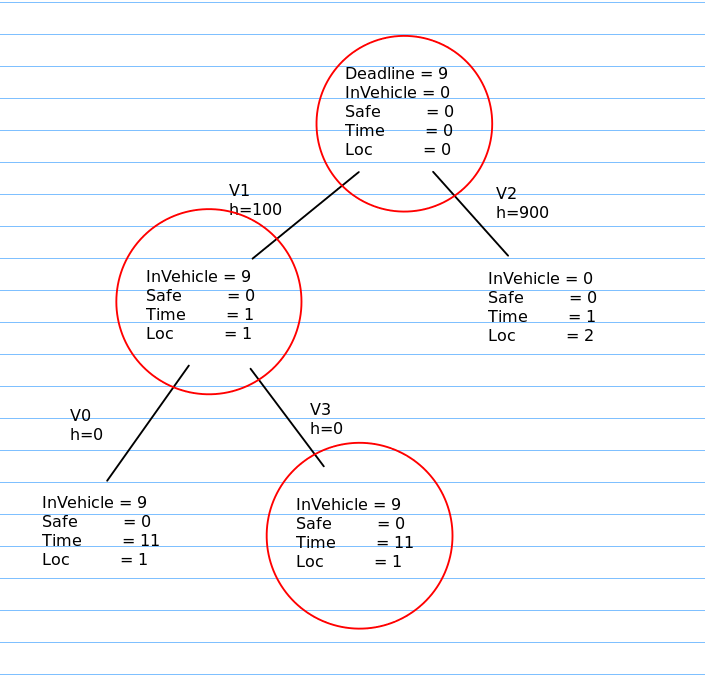
\includegraphics[width=0.5\linewidth]{q2a}
		\caption{Greedy agent expansions}
		\label{fig:q2a}
	\end{figure}
	
	
	\subsection{$ A^* $}
	Opposed to the greedy agent, the $ A^* $ agent will provide an optimal solution, although the heuristic is not admissible. This is due to the fact that the g value is complementary. Since, the heuristic is extremely optimistic the $ A^* $ agent will perform much more expansions than he would have needed if the heuristic was better.
	
	The $ A^* $ agent takes into account the time took to get to this state, and if a goal state is reached it adds the number of unsaved  people.
	\begin{equation}\label{eq:g_val}
		g_{v_i\rightarrow v_j}=
		\begin{cases}
		g[v_i] + w_{v_iv_j},& t + w_{v_iv_j} < T_{deadline}\\
		g[v_i] + w_{v_iv_j} + 100\times UnsavedPeople,& else\\
		\end{cases}
	\end{equation} 
	The agent adds the $ g $ value with the $ h $ value to decide which node to expand.
	
	Fig. \ref{fig:q2b} shows the expansion tree of the $ A^* $ agent. It can be seen that the agent has 11\footnote{The state $ V_0 $ with f=902 was not expanded since it is assumed there is a checking for loops to avoid expanding already visited states.} expansions to find the optimal path, which is $ V_0\rightarrow V_2\rightarrow V_3\rightarrow V_2\rightarrow V_0$. 

	
	\begin{figure}
		\centering
		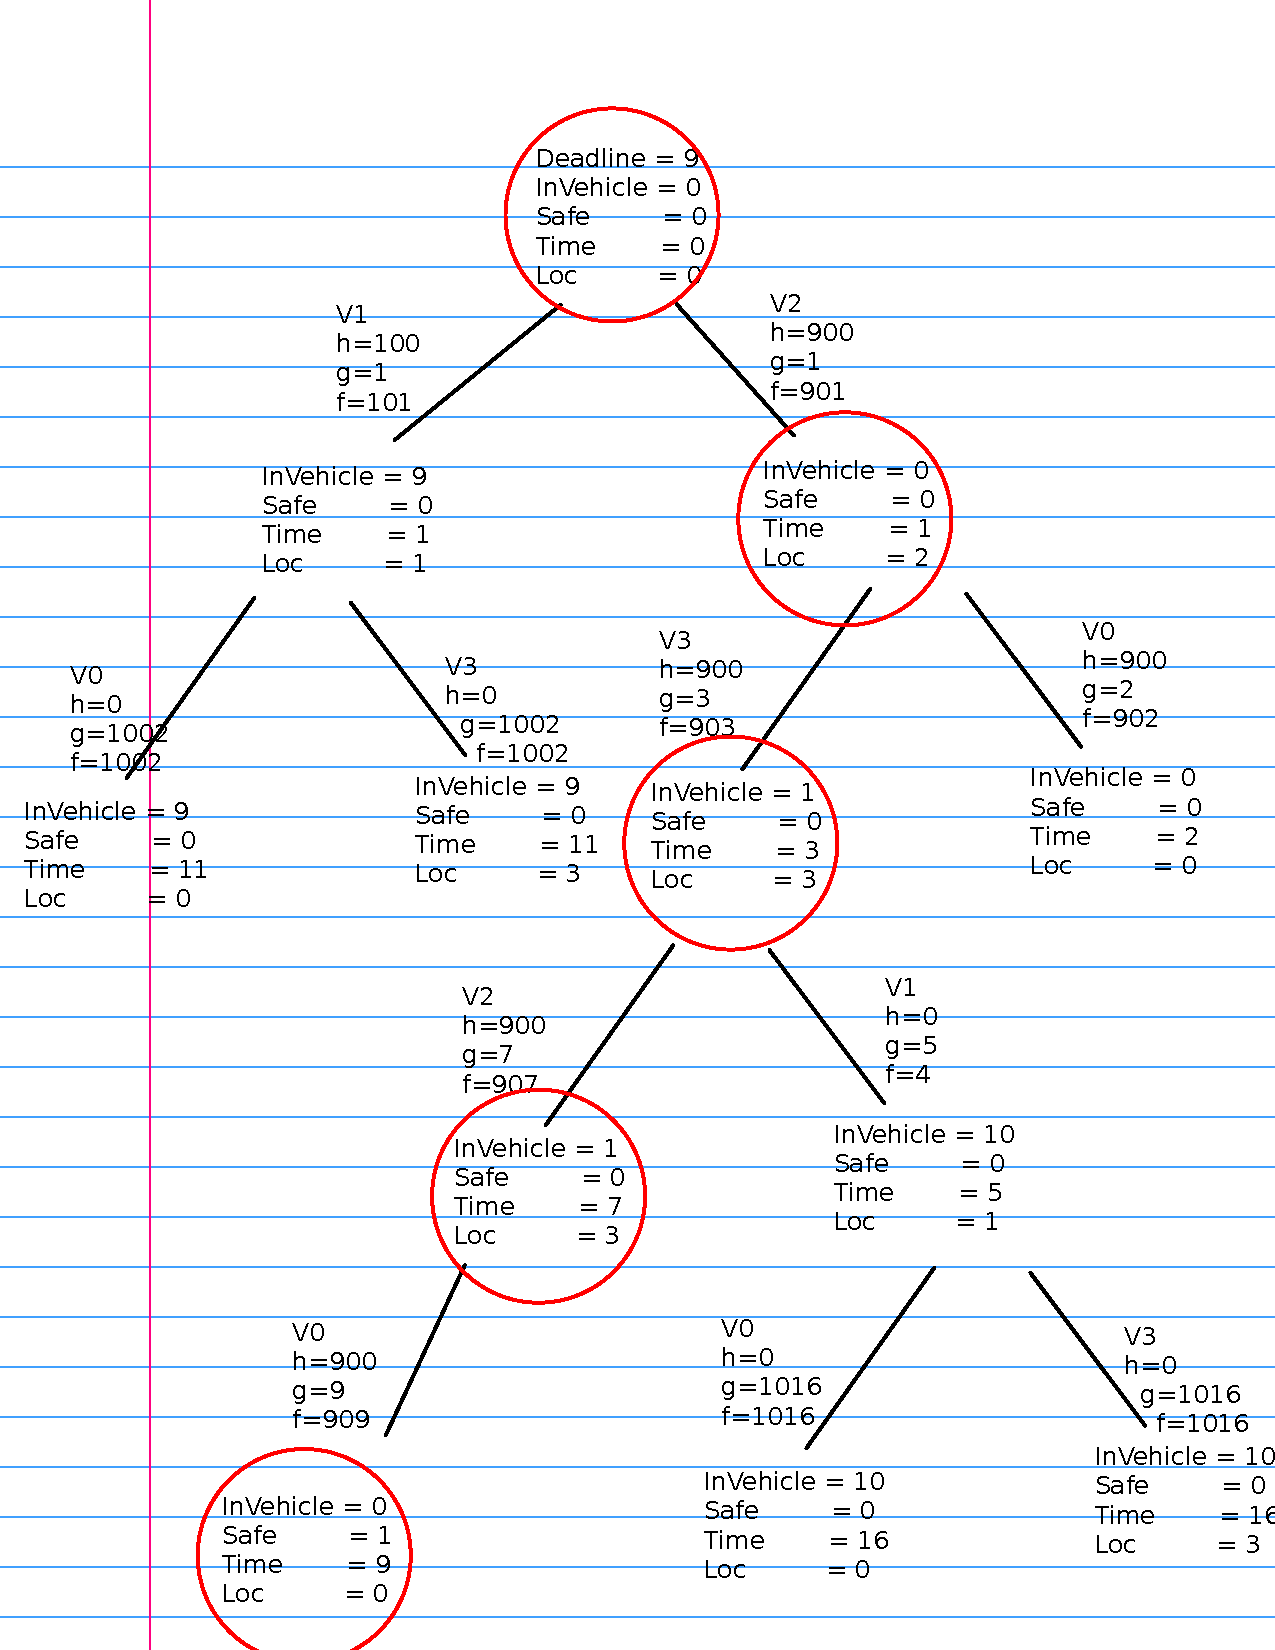
\includegraphics[width=0.5\linewidth]{q2_b}
		\caption{$ A^* $ agent expansions}
		\label{fig:q2b}
	\end{figure}

	\subsection{Real-time $ A^* $}
	
	This agent is similar to the $ A^* $ agent, however, it stops after 2 expansions and makes a decision. Fig~\ref{fig:q2c1} shows the first two expansions of the agent. It can be seen that in this case, the same result state is achieved as with the the $ A^* $ agent. After the agent reached $ V_3 $ the agent expanded up to two more nodes, as shown in Fig.~\ref{fig:q2c2}.
	\begin{figure}
		\centering
		\begin{subfigure}[b]{0.4\textwidth}
			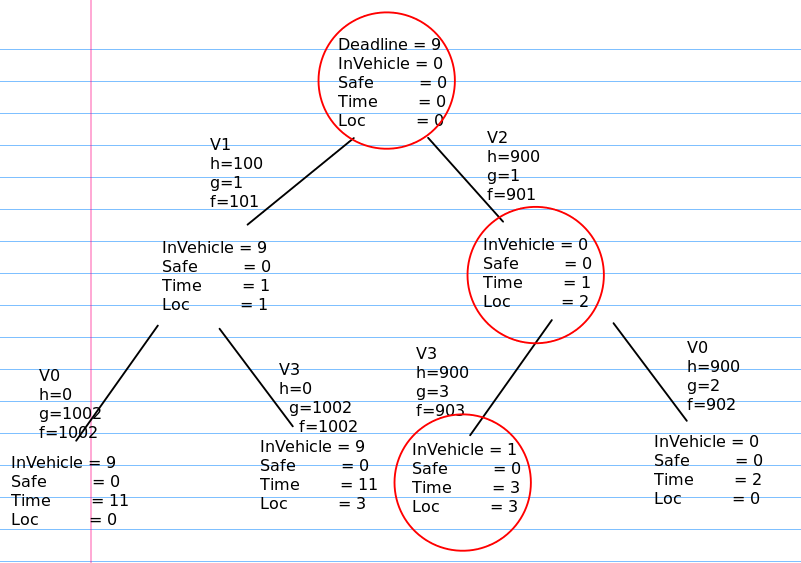
\includegraphics[width=\textwidth]{q2_c_1}
			\caption{Real-Time $ A^* $ agent first 2 expansions.}
			\label{fig:q2c1}
		\end{subfigure}
		\begin{subfigure}[b]{0.4\textwidth}
			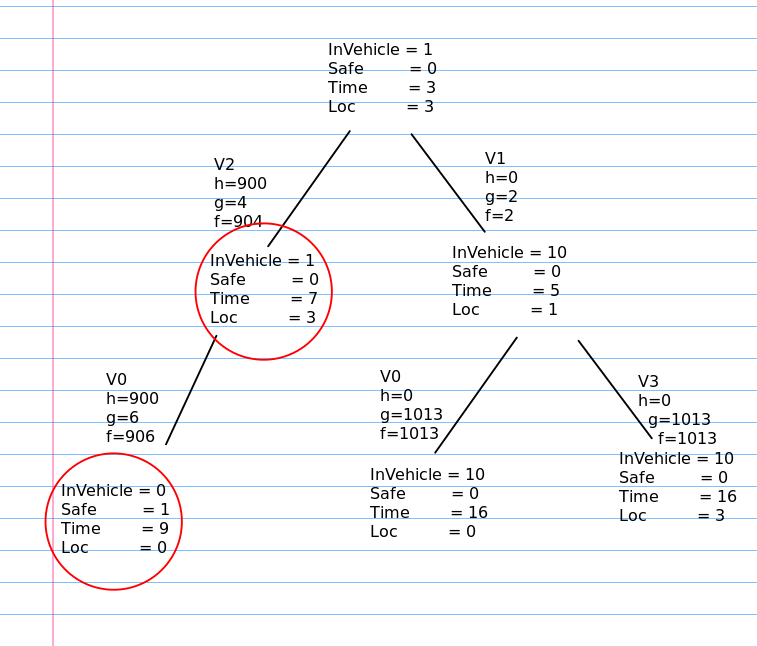
\includegraphics[width=\textwidth]{q2_c_2}
			\caption{Real-Time $ A^* $ agent second 2 expansions.}
			\label{fig:q2c2}
		\end{subfigure}
	
	\end{figure}

	\subsection{$ h=2 * h' $}
	Since $ h' $ multiplied the number of people by a large number, it does not matter if this large number is $ X $ or $ 2*X $. Therefore, all of the results will remain the same, and the heuristic is still admissible.
	
	\section{Game trees}
	\subsection{Each agent out for itself, and they cannot communicate.}
	\begin{figure}[H]
		\centering
		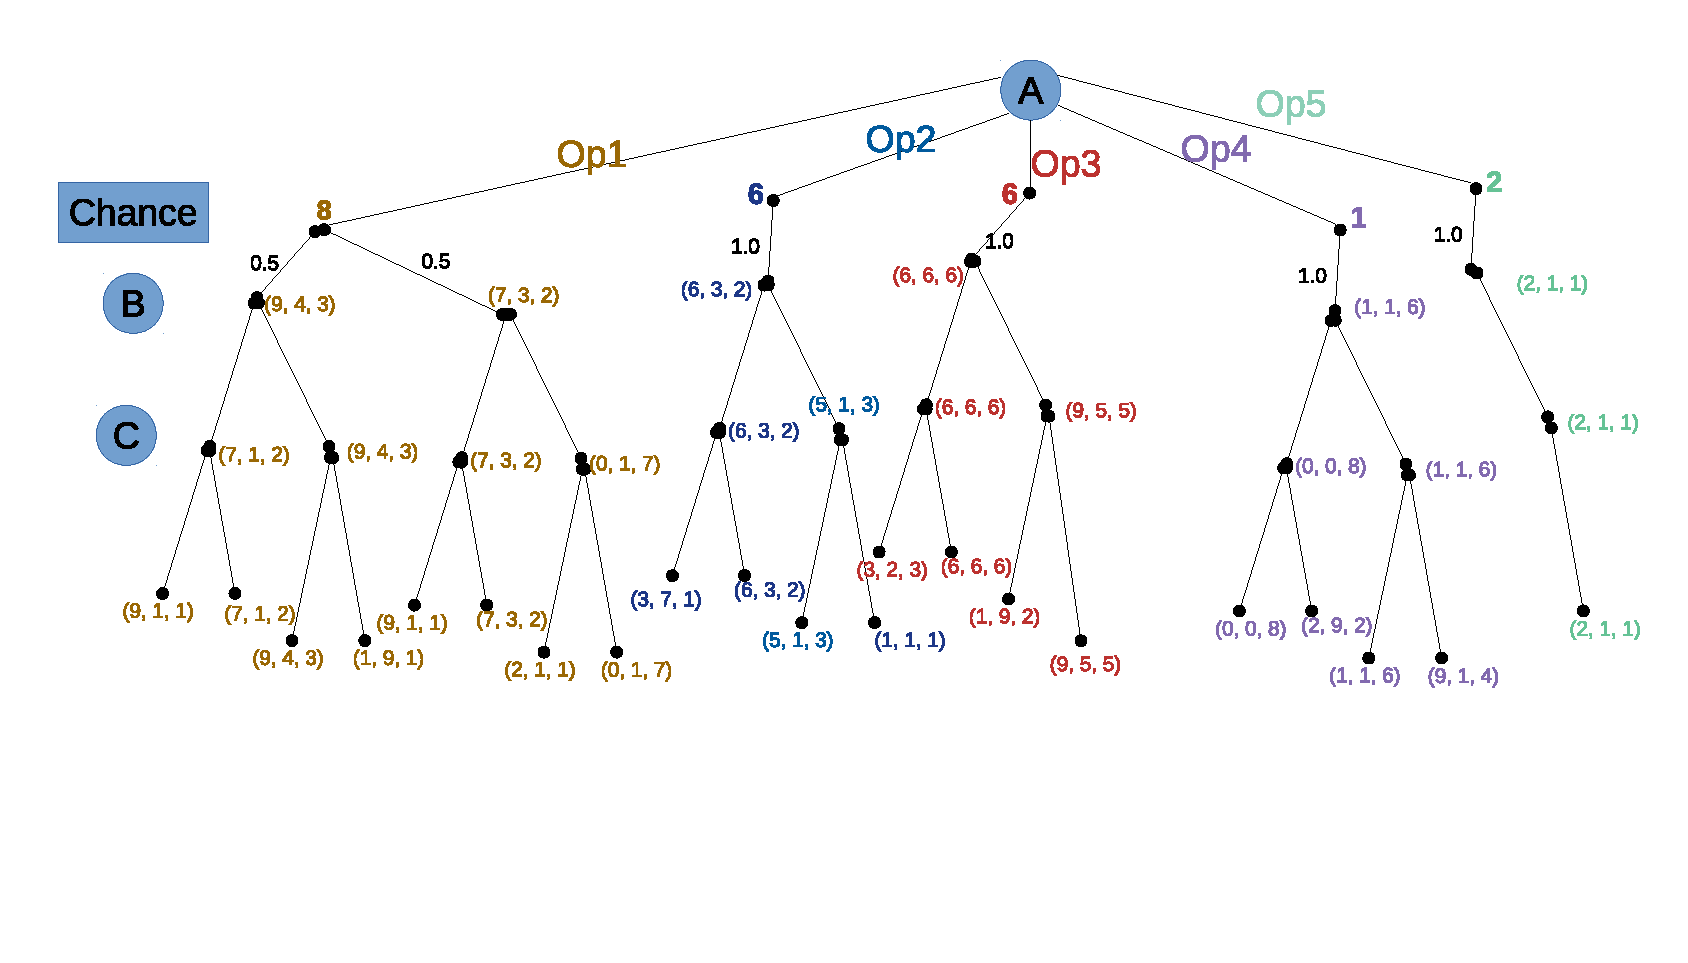
\includegraphics[width=0.7\linewidth]{q3_1.eps}
		\caption{Option 1 is the best}
		\label{fig:q31}
	\end{figure}
	
	\subsection{Paranoid assumption: B and C are against A}
	\begin{figure}[H]
		\centering
		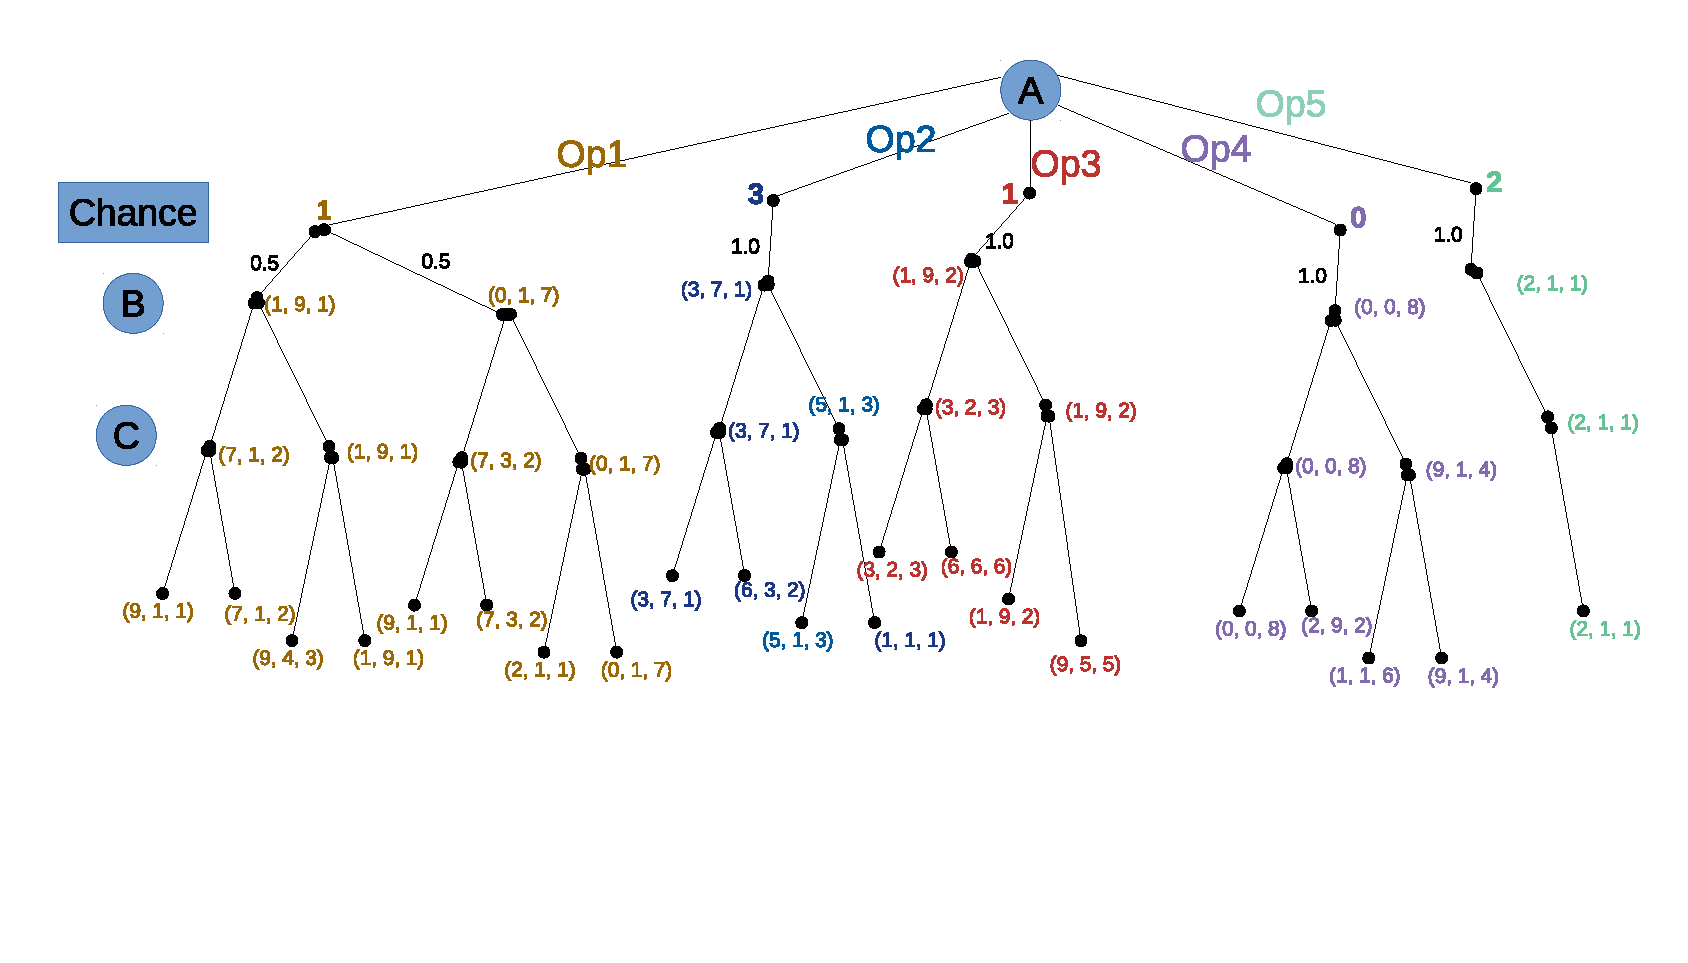
\includegraphics[width=0.7\linewidth]{q3_2.eps}
		\caption{Option 2 is the best}
		\label{fig:q31}
	\end{figure}

	\subsection{B and C may agree on a deal if it is beneficial to both of them}
	\begin{figure}[H]
		\centering
		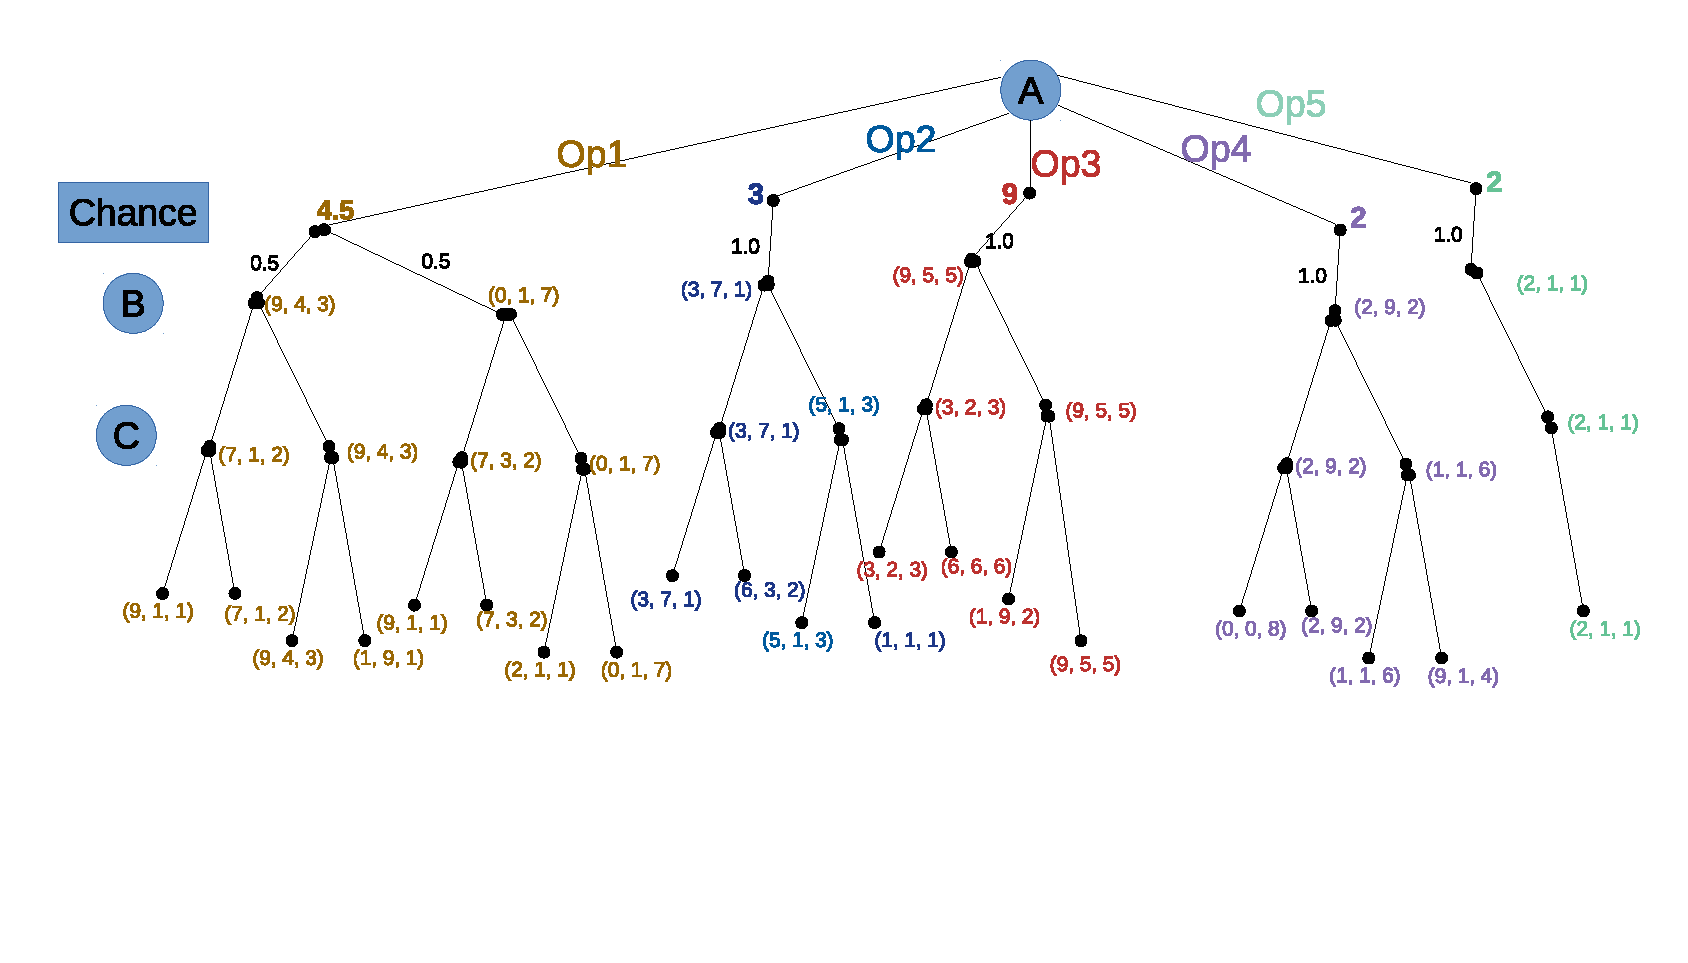
\includegraphics[width=0.7\linewidth]{q3_3.eps}
		\caption{Option 3 is the best}
		\label{fig:q31}
	\end{figure}

	\subsection{A and C are partners aiming to maximize the sum of their scores}
	\begin{figure}[H]
		\centering
		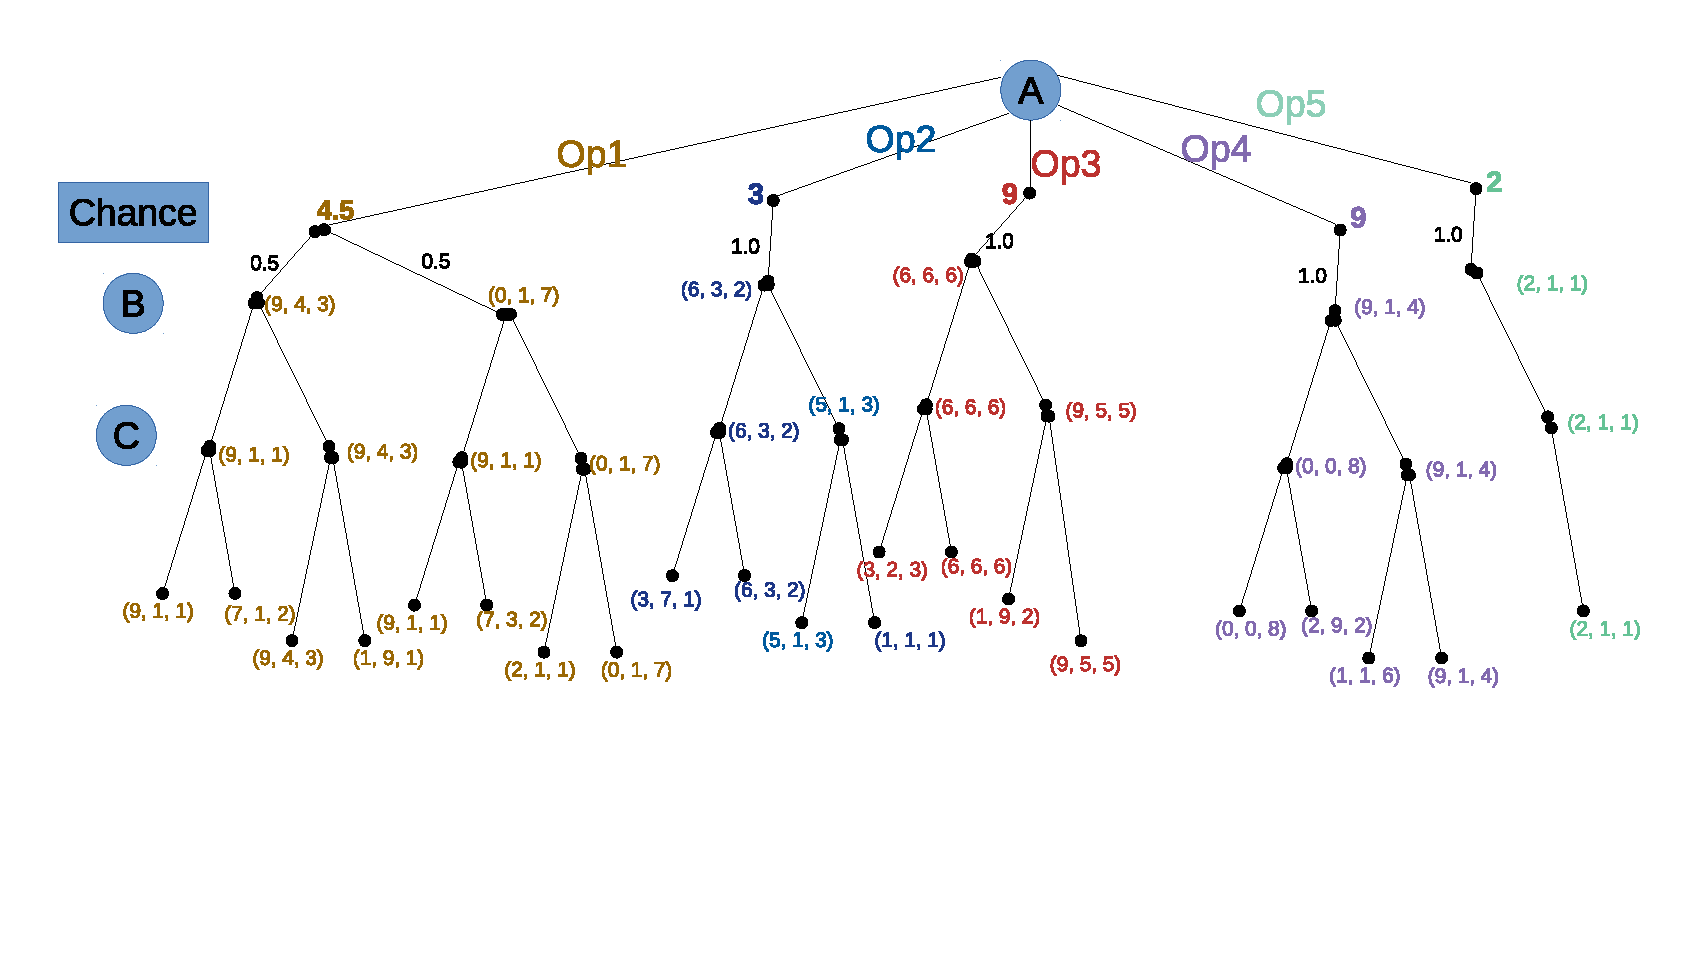
\includegraphics[width=0.7\linewidth]{q3_4.eps}
		\caption{Option 4 is the best}
		\label{fig:q31}
	\end{figure}

	\subsection{A is a firm believer in Murphy's laws: "mother nature is a b*!=h", and wants toplay absolutely safe.}
	\begin{figure}[H]
		\centering
		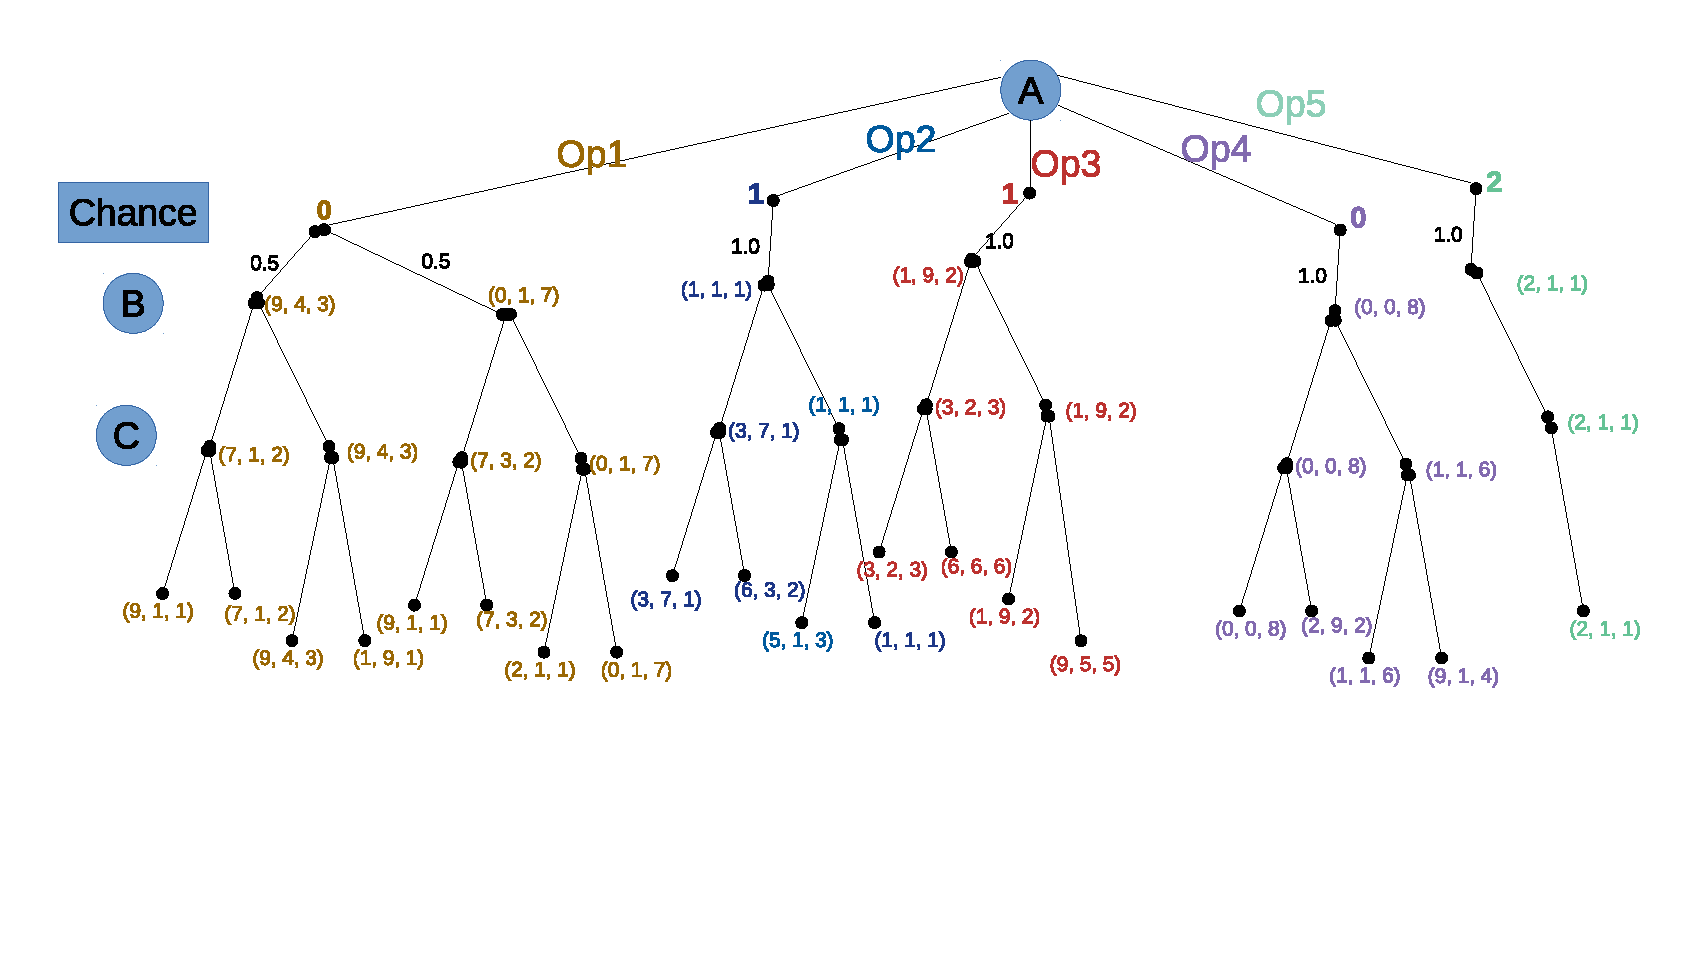
\includegraphics[width=0.7\linewidth]{q3_5.eps}
		\caption{Option 5 is the best}
		\label{fig:q31}
	\end{figure}

	
	\section{Game-tree search - alpha-beta pruning}
	
	
	\section{Propositional logic}
	For validity it will be shown that the sentence is always true.
	
	An example for satisfiability a true model and a false model will be given.
	
	For unsatisfiability it will be shown that the setence is always false.
	
	Number of models equals to: $ 2^n $, if the sentence is valid, where n is the number of symbols.
	
	\subsection{$ (\nt{A} \land \nt{B} \land \nt{C} \land \nt{D} \land \nt{E} \land F) \lor (A \land B \land C \land D \land E)$}
	\textit{True model} - A, B, C, D, F are true, therefore,
	
	$ True \lor False = True$
	
	\textit{False model} - A is true, B is false (the rest whatever), therefore,

	$ False \lor False = False $
	
	\textbf{Satisfiable}. Number of satisfiable models is 3.
	\subsection{$ (\nt{A} \lor \nt{B} \lor \nt{C} \lor \nt{D} \lor \nt{E} \lor \nt{F}) \land (A \lor B \lor C \lor D \lor E \lor F)$}
	\textit{False model} - A, B, C, D, F are true, therefore,
	
	$ True \land False = False$
	
	\textit{True model} - A is true, B is false (the rest whatever), therefore,
	
	$ True \land True = True $
	
	\textbf{Satisfiable}. Number of satisfiable models is 62.
	
	\subsection{$ (A \lor B \land (D \lor \nt{A}) \land (E \lor A) \Rightarrow  (B \lor C \land (\nt{D} \lor E))) \land (A \land \nt{A})$}
	
	$ \alpha \equiv (A \lor B \land (D \lor \nt{A}) \land (E \lor A) \Rightarrow  (B \lor C \land (\nt{D} \lor E))) $
	
	
	$ \alpha \land (A \land \nt{A}) \rightarrow \alpha \land False \rightarrow False $
	
	\textbf{Unsatisfiable}  Number of models is 0.
	
	\subsection{$ (A \land (A \Rightarrow B) \land (B \Rightarrow C)) \Rightarrow C $}

	\begin{description}
		\item [implication elimination]
		$ \neg (A \land (\nt{A} \lor B) \land (\nt{B} \lor C)) \lor C  $
		\item [Distributivity]
		$ \neg ((A \land \nt{A}) \lor (A \land B)) \land (\nt{B} \lor C)) \lor C  $
		
		$ \neg (False \lor (A \land B)) \land (\nt{B} \lor C)) \lor C  $
		\item [Associativity]
		$ \neg (A \land (B \land (\nt{B} \lor C))) \lor C  $
		\item [Distributivity]
		$ \neg (A \land ((B \land \nt{B}) \lor (B \land C))) \lor C  $
		
		$ \neg (A \land ((False) \lor (B \land C))) \lor C  $

		$ \neg (A \land (B \land C)) \lor C  $
		\item[De Morgan]
		$ \nt{A} \lor \nt{B} \lor \nt{C} \lor C \rightarrow True $
	\end{description}

		\textbf{Valid}.  Number of models is 8.

	\subsection{$ \neg ((A \land (A \Rightarrow B) \land (B \Rightarrow C)) \Rightarrow C )$}
	\begin{description}
		\item[implication elimination] 	$ \neg (\neg(A \land (\nt{A} \lor B) \land (\nt{B} \land C)) \lor C )$
		\item[Distributivity]  $ \neg (\neg((A \land \nt{A}) \lor (A \land B) \land (\nt{B} \land C)) \lor C )$
		
		$ \neg (\neg((A \land B) \land (\nt{B} \land C)) \lor C )$
		\item[De Morgan] 		$ \neg (\nt{A} \lor \nt{B} \lor \nt{\nt{B}} \lor \nt{C} \lor C )$
		\item[Double negation elimination] $ \neg (\nt{A} \lor \nt{B} \lor B \lor \nt{C} \lor C ) \rightarrow $
		
		$ \neg (\nt{A} \lor True \lor True ) \rightarrow$
		
		$ \neg (True) \rightarrow False$
	\end{description}

	\textbf{Unsatisfiable}.  Number of models is 0.
	
	\subsection{$ (A\Rightarrow \nt{A}) \lor (\nt{A} \Rightarrow A) $}
		\begin{description}
		\item[implication elimination] $ (\nt{A} \lor \nt{A}) \lor (A \lor A) \rightarrow $
		
		$ \nt{A} \lor A \rightarrow True$
		
	\end{description}

	\textbf{Valid}.  Number of models is 2.
	
	
	\section{FOL and situation calculus}		

	\subsection{Axioms of world behavior}
	
	\subsubsection{Auxiliary predicats }
	\begin{itemize}
		\item TimeUp(s) - check if time passed the deadline
		
\begin{equation}\label{key}
		 \forall s, t \exists d \quad TimeUp(s) \Rightarrow Time(t, s) > Deadline(d) 
\end{equation}
		
		\item Bidirectional edge
		\begin{equation}\label{key}
		 \forall e, v1, v2 \quad Edge(e, v1, v2) \Leftrightarrow Edge(e, v2, v1) 
		\end{equation}
		
	\end{itemize}


	\subsubsection{Effect axioms}
	\begin{itemize}
		
		
		
		\item Update time fluent
		\begin{equation}\label{key}
		\forall a, s, t \quad  
		(\exists e, w \quad a=Traverse(e) \land Weight(e, w)) \land Time(t, s)
		\Rightarrow 
		Time(t+w, Result(a, s))
		\end{equation}
		or,
\begin{equation}\label{key}
		\forall at, a, s, t \quad  
		a=NoOp() \land Time(t, s)
		\Rightarrow 
		Time(t+1, Result(a, s))
\end{equation}
		
				
		\item Loc update
		\begin{equation}\label{key}
		\forall s, v1, a, e \quad (\exists v \quad a=Traverse(e) \land Edge(e, v, v1) \land Loc(v, s)) \Rightarrow Loc(v1, Result(a, s))
		\end{equation}
		
		\item Pickup people
		\begin{equation}\label{key}
		 \forall c, v, a, s \quad Carrying(c ,s)\land Loc(v, Result(a, s)) \Rightarrow \exists n At(v, n, s) \land Carrying(c + n, Result(a, s))  
		\end{equation}
		\item Remove picked up people
		
		For all states and vertices, 0 people are at vertex, v, if loc is v.
\begin{equation}\label{key}
		 \forall v, a, s \quad Loc(v, Result(a, s)) \Rightarrow  At(v, 0, Result(a, s))
\end{equation}
		
		\item Save people
		
		People in vehicle are safe if vehicle is at a shelter and time is not up
		\begin{equation}\label{key}
		 \forall s, a, v, n \quad Safe(n, s) \land Loc(v, s) \land Shelter(v) \land \nt{TimeUp(s)} \Rightarrow \exists c\quad Safe(n + c, Result(a, s))\land Carrying(c, s)  
		\end{equation}
		
		\item Remove carried people
		\begin{equation}\label{key}
		 \forall s, a, v \quad Loc(v, s) \land Shelter(v) \land \nt{TimeUp(s)} \Rightarrow Carrying(0, Result(a, s))  
		\end{equation}				
	\end{itemize}


	
	\subsubsection{Successor state axioms}
	\begin{itemize}
		\item Loc unchanged
		
		\begin{equation}\label{key}
		\forall a, s, v  \quad Loc(v, s) \Leftrightarrow Loc(v, Result(a, s)) \land (a = NoOp())
		\end{equation}
		
		
		\item Number of people in towns unchanged
		 \begin{equation}\label{key}
		\forall a, v, s\quad  At(v, n, s) \land \nt{Loc(v, s)} \Rightarrow At(v, n, Result(a, s))
		\end{equation} 
		
		\item Number of safe people unchanged
		 \begin{equation}\label{key}
		\forall a, s \quad   Safe(n, s) + (\exists v\quad (Loc(v, s) \land \neg Shelter(v) ) \Rightarrow Safe(n, Result(a, s))
		\end{equation}
		
		\item Number of people carrying unchanged
		 \begin{equation}\label{key}
		\forall a, s \quad Carrying(n, s) \land (\exists v \quad (Loc(v, s) \land \nt{Shelter(v)}) \Rightarrow  Carrying(n, Result(a, ∨ ∃(cs))
		\end{equation}
	\end{itemize}
	

	\subsection{Prove that the people in V3 are safe}

	Please note - This is an extremely long process. Therefore, all the NoOp are not written since they are not part of the plan. In addition, simple arithmetic, which should be part of the axioms are excluded. 
	\subsubsection{CNF}
	
	\begin{equation}\label{cnf:timeup}
	\forall s, t \exists d \quad \neg TimeUp(s) \lor (Time(t, s) > Deadline(d))
	\end{equation}	
	
	\begin{equation}\label{cnf:edge}
	\forall e, v1, v2 (\neg Edge(e, v1, v2) \lor Edge(e, v2, v1)) \land (Edge(e, v1, v2) \lor \neg Edge(e, v2, v1))
	\end{equation}
	 
	\begin{equation}\label{cnf:time_update}
	\forall a, s, t \quad  
	(\forall e, w \quad \neg a=Traverse(e) \lor \neg Weight(e, w)) \lor \neg Time(t, s)
	\lor 
	Time(t+w, Result(a, s))
	\end{equation}
	
	
	$$ \forall s, v1, a, e \quad (\neg\exists v \quad a=Traverse(e) \land Edge(e, v, v1) \land Loc(v, s)) \lor Loc(v1, Result(a, s))$$
	\begin{equation}\label{cnf:loc_update}
	\forall s, v1, a, e \quad (\forall v \quad \neg (a=Traverse(e)) \lor \neg Edge(e, v, v1) \lor \neg Loc(v, s)) \lor Loc(v1, Result(a, s))
	\end{equation}
	
	
	\begin{equation}\label{cnf:pick_update}
	\forall v, a, s, c \quad \neg Carrying(c, s) \neg Loc(v, Result(a, s)) \lor (\exists n \quad Carrying(n + c, Result(a, s)) \land At(v, n, s))
	\end{equation}

	\begin{equation}\label{cnf:remove_pickup}
	\forall v, a, s \quad \neg Loc(v, Result(a, s)) \lor  At(v, 0, Result(a, s))
	\end{equation}
	
	\begin{equation}\label{cnf:safe}
	\neg Safe(n, s) \lor \neg Loc(v, s) \lor \neg Shelter(v) \lor {TimeUp(s)} \lor \exists (c\quad Safe(n + c, Result(a, s))\land Carrying(c, s))
	\end{equation}
	
	\begin{equation}\label{cnf:rm_carried}
	\forall s, a, v \quad	\neg Loc(v, s) \lor \neg Shelter(v) \lor TimeUp(s) \lor Carrying(0, Result(a, s))
	\end{equation}
	
	\begin{equation}\label{cnf:at_unc}
 	\forall a, v, s\quad At(v, n, Result(a, s)) \lor \neg At(v, n, s) \lor \nt{Loc(v, s)}
	\end{equation}
	
	\begin{equation}\label{cnf:safe_unc}
	\forall a, v, n, s\quad \neg Safe(n,s) \lor \neg Loc(v,s) \lor Shelter(v) \lor Safe(n, Result(a, s))
	\end{equation}
	
	\begin{equation}\label{pick_unc}
	 \forall v, a, s \quad \neg Carrying(c, s) \lor \neg Loc(v, Result(a, s)) \lor Shelter(v) \lor Carrying(n, Result(a, s))) 
	\end{equation}
	
	

	
	
	
	
	\subsubsection{What we need to prove}
	From Q2 we have discovered that the optimal plan is $ E2 \rightarrow E3 \rightarrow E3 \rightarrow E2 $, and the location of the agent will be $ V0 \rightarrow V2 \rightarrow V3 \rightarrow V2 \rightarrow V0$.
	
	In order to show this plan, $ p=[Traverse(E2), Traverse(E3), Traverse(E3), Traverse(E2)] $ will actually save the people in $ V3 $, we shall prove by contradiction that time will not elapse, i.e. $ KB \land p \land TimeOut(S4) $ is false. In addition, we shall prove that the people are actually safe, i.e., $ KB \land p \land (\exists n \quad \neg(Safe(n, S4)\land At(V3, n, s0))) $
	
	\subsubsection{Proof with resolution}
\begin{equation}\label{res:s1}
	 S1 = Result(Traverse(E2), S0) 
\end{equation}
\begin{equation}\label{res:s2}
	 S2 = Result(Traverse(E3), S1) 
\end{equation}
\begin{equation}\label{res:s3}
	 S3 = Result(Traverse(E3), S2) 
\end{equation}
\begin{equation}\label{res:s4}
	 S4 = Result(Traverse(E2), S3) 
\end{equation}
\begin{equation}\label{res:Timeout}
	 TimeOut(S4) 
\end{equation}
	
\begin{equation}\label{res:l0}
	 Loc(V0, S0)  
\end{equation}
\begin{equation}\label{res:c0}
	 Carrying(0, S0)  
\end{equation}
\begin{equation}\label{res:at0}
	 At(V3, 1, S0)  
\end{equation}
\begin{equation}\label{key}
	 At(V1, 9, S0)   
\end{equation}
\begin{equation}\label{res:safe0}
	 Safe(0, S0)  
\end{equation}
\begin{equation}\label{res:t0}
	 Time(0, S0)  
\end{equation}
\begin{equation}\label{res:deadline}
Deadline(9)
\end{equation}
	
	And more...
	
	1. Proof of Timeup
	Resolving \ref{cnf:timeup} and \ref{res:Timeout} and \ref{res:deadline}
	\begin{equation}\label{cnf:timeout}
	TimeUp(S4), Deadline(9), \neg TimeUp(s) \lor (Time(t, s) > Deadline(d)) \rightarrow
	\end{equation}
	$$ Time(t, S4) > Deadline(9) $$
	
	Resolving \ref{cnf:time_update} and \ref{res:at0} and Weight(E2,2) and \ref{res:s1}
	\begin{equation}\label{res:t1}
	\begin{split}
	Time(0, S0), S1 = Result(Traverse(E2), S0), Weight(E2,2), \\
	 \neg a=Traverse(e) \lor \neg Weight(e, w)) \lor \neg Time(t, s)
	\lor 
	Time(t+w, Result(a, s))
	\end{split}
	\end{equation}
	$$ Time(0+2, S1) \rightarrow Time(2, S1) $$
	
	Resolving \ref{cnf:time_update} and \ref{res:t1} and Weight(E3,2) and \ref{res:s2}
	\begin{equation}\label{key}
	\begin{split}
	Time(1, S1), S2 = Result(Traverse(E3), S1), Weight(E3,1),  \\
	\neg a=Traverse(e) \lor \neg Weight(e, w)) \lor \neg Time(t, s)
	\lor 
	Time(t+w, Result(a, s))
	\end{split}
	\end{equation}	
	$$ Time(2+1, S2) \rightarrow Time(3, S2) $$	

	\begin{equation}\label{key}
	\begin{split}
	Time(3, S3), S3 = Result(Traverse(E3), S2), Weight(E3,1),  \\
	\neg a=Traverse(e) \lor \neg Weight(e, w)) \lor \neg Time(t, s)
	\lor 
	Time(t+w, Result(a, s))
	\end{split}
	\end{equation}	
	$$ Time(3+1, S3) \rightarrow Time(4, S3) $$	

	\begin{equation}\label{key}
	\begin{split}
	Time(4, S3), S2 = Result(Traverse(E2), S3), Weight(E2,2),  \\
	\neg a=Traverse(e) \lor \neg Weight(e, w)) \lor \neg Time(t, s)
	\lor 
	Time(t+w, Result(a, s))
	\end{split}
	\end{equation}	
	$$ Time(4+2, S4) \rightarrow Time(6, S4) $$	
	
	From CNF \ref{cnf:timeout} and the Time expansion above we get a contradiction, i.e.,
	\begin{equation}\label{key}
	\begin{split}
		Time(6, S4), Time(t, S4) > Deadline(9) \Rightarrow False
	\end{split}
	\end{equation}
	
	This concludes that time does not elapse. We will continue with proving the people are safe.
	
	2. Proof of safety
	$$ \exists n \quad \neg(Safe(n, S4)\land At(V3, n, s0)) $$
	$$ \exists n \quad \neg Safe(n, S4)\lor \neg At(V3, n, s0) $$
	
	Along with At(V3, 1, S0) we need to disprove that,
	$$ \neg Safe(1, S4) $$
	
	\begin{equation}\label{key}
	\begin{split}
	S1 = Result(Traverse(E2), S0), Loc(V0, S0), Edge(E2, V0, V2),  \\\neg (a=Traverse(e)) \lor \neg Edge(e, v, v1) \lor \neg Loc(v, s)) \lor Loc(v1, Result(a, s))
	\end{split}
	\end{equation}
	$$ Loc(V2, S1) $$
	
	\begin{equation}\label{key}
	\begin{split}
	S2 = Result(Traverse(E3), S1), Loc(V2, S1), Edge(E3, V2, V3),  \\\neg (a=Traverse(e)) \lor \neg Edge(e, v, v1) \lor \neg Loc(v, s)) \lor Loc(v1, Result(a, s))
	\end{split}
	\end{equation}
	$$ Loc(V3, S2) $$
	
	\begin{equation}\label{key}
	\begin{split}
	S3 = Result(Traverse(E3), S2), Loc(V3, S2), Edge(E3, V2, V3),  \\\neg (a=Traverse(e)) \lor \neg Edge(e, v, v1) \lor \neg Loc(v, s)) \lor Loc(v1, Result(a, s)), and \eqref{cnf:edge}
	\end{split}
	\end{equation}
	$$ Loc(V2, S3) $$
	
	\begin{equation}\label{key}
	\begin{split}
	S4 = Result(Traverse(E2), S3), Loc(V2, S3), Edge(E2, V0, V2), \\ \neg (a=Traverse(e)) \lor \neg Edge(e, v, v1) \lor \neg Loc(v, s)) \lor Loc(v1, Result(a, s)), and \eqref{cnf:edge}
	\end{split}
	\end{equation}
	$$ Loc(V0, S4) $$
	
	In addition, we need to move the At() fluents forward for all cases, but we will show only for V3 using \ref{cnf:at_unc}
	\begin{equation}\label{key}
	\begin{split}
	S1 = Result(Traverse(E2), S0), At(V3, 1, S0), Loc(V0, S0),	 \\At(v, n, Result(a, s)) \lor \neg At(v, n, s) \lor \nt{Loc(v, s)} \rightarrow
	\end{split}
	\end{equation}
	$$ At(V3, 1, S1) $$
	
	\begin{equation}\label{key}
	\begin{split}
	S2 = Result(Traverse(E3), S1), At(V3, 1, S1), Loc(V2, S1),	 \\At(v, n, Result(a, s)) \lor \neg At(v, n, s) \lor \nt{Loc(v, s)} \rightarrow
	\end{split}
	\end{equation}
	$$ At(V3, 1, S2) $$
	
	At next state \eqref{cnf:at_unc} will not hold, however, \eqref{cnf:remove_pickup} does hold, and thus,
	\begin{equation}\label{key}
	\begin{split}
	S3 = Result(Traverse(E3), S2), At(V3, 1, S2), Loc(V3, S2),	 \\\neg Loc(v, Result(a, s)) \lor  At(v, 0, Result(a, s)) \rightarrow
	\end{split}
	\end{equation}
	$$ At(V3, 0, S3) $$
	
	Now we need to handle the carrying fluent. The same procedure is applied as with the At fluent. To conserve time and space, we will skip this process and jump to the fluent at state S4, i.e., 
	$$ Carrying(1, S4) $$
	
	The final step for proving the people are safe is performed using \eqref{cnf:safe}. Once again, we skipped propagating the safe fluent through states.
	
	\begin{equation}\label{key}
	\begin{split}
	Safe(0, S3), S4=Result(Tranverse(E2), S3), Loc(v0, S4), Shelter(V0), \neg TimeUp(S4), Carrying(1, S4) \\
	\neg Safe(n, s) \lor \neg Loc(v, s) \lor \neg Shelter(v) \lor {TimeUp(s)} \lor \exists (c\quad Safe(n + c, Result(a, s))\land Carrying(c, s))
	\end{split}
	\end{equation}
	$$ 	Safe(1, S4) $$
	
	We got a contradiction, therefore, the people are safe and sound. 
	
	

	\subsection{Remove frame axioms - bad idea}
	Of course the proof will fail without the frame (Successor state) axioms since we won't have any knowledge of whether there are people at $ V_3 $ any more, or will not know what if people are safe, or are we carrying people in the vehicle.
	
	\subsection{Proving with forward chaining}
	Unfortunately, Forward chaining is not an option since there are some non Horn clauses (e.g. \eqref{cnf:safe}) where more than one of the predacits is positive. 

\end{document}

